\documentclass{article}
\usepackage[T1]{fontenc}
\usepackage{lmodern}
\usepackage{graphicx}
\usepackage{amsmath,amssymb}
\usepackage[a4paper,margin=2cm]{geometry}
\usepackage[absolute,overlay]{textpos}
\setlength{\TPHorizModule}{1mm}
\setlength{\TPVertModule}{1mm}
\usepackage[indonesian]{babel}
\usepackage{hyperref}
\setlength{\emergencystretch}{2em}
% unit: Halaman 20

\begin{document}

% === Halaman 20 (llm) ===

\vspace{163.35mm}

Contoh:\vspace{50mm}
Proses substitusi 23 menjadi 26

% deskripsi: Ilustrasi transisi antara dua state berupa matriks 4x4 dengan panah di antaranya, menunjukkan perubahan nilai tertentu.
% bbox normalisasi: [0.1900, 0.2100, 0.6500, 0.3100]
\begin{textblock*}{96.60mm}(39.90mm,62.37mm)
\noindent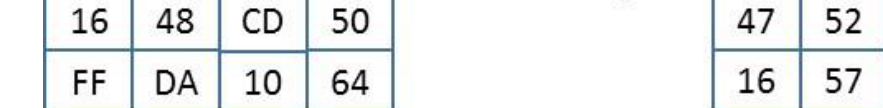
\includegraphics[width=96.60mm,height=29.70mm]{../../images/llm/page_020_img_01.png}%
\end{textblock*}

% deskripsi: Tabel substitusi S-Box yang berisi pemetaan nilai heksadesimal dari baris 0-F dan kolom 0-F.
% bbox normalisasi: [0.1800, 0.3700, 0.7900, 0.9200]
\begin{textblock*}{128.10mm}(37.80mm,109.89mm)
\noindent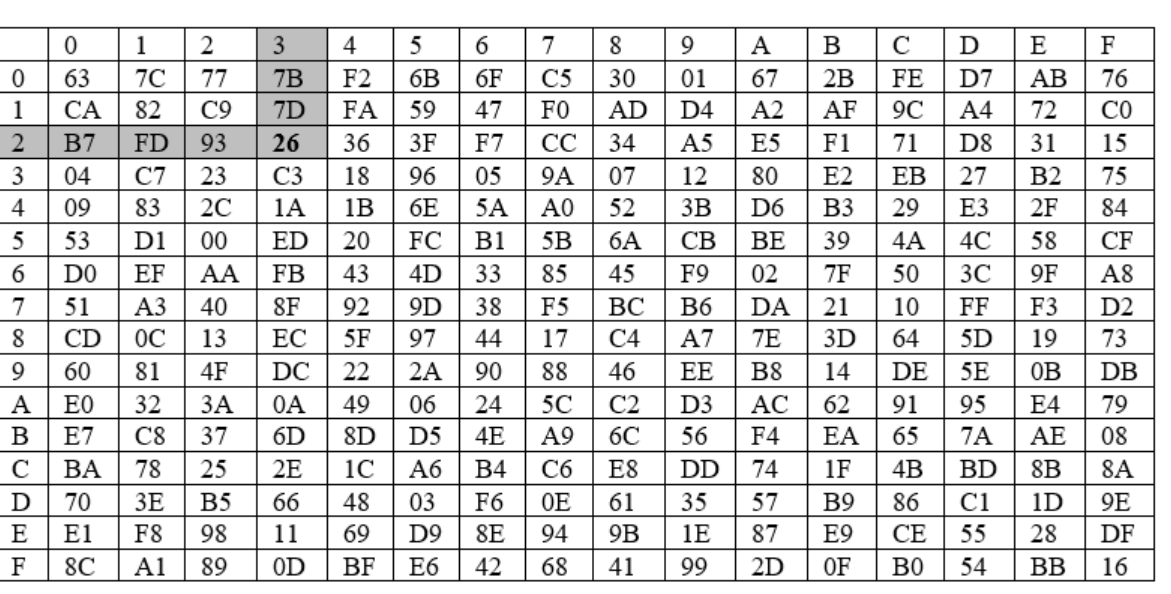
\includegraphics[width=128.10mm,height=163.35mm]{../../images/llm/page_020_img_02.png}%
\end{textblock*}

\end{document}
